\chapter{How to Write Descriptively}

This lecture begins from the reader's side and only then turns toward craft. We ask first why fiction matters, then what prose must do if it is to absorb us as strongly as lived experience, theater, or film. The central claim is that descriptive language is not decoration laid over a story. It is one of the mechanisms by which static marks on a page become sensation, association, and finally immersion.

\section{Why We Read Fiction, and Why Description Matters}

The opening list is deliberately broad. We read fiction to be entertained, to find out who did it, to travel to strange new worlds, to be scared, to laugh, to cry, to think, and to feel. But the lecture does not leave us with a catalogue of motives. It drives toward the strongest one: we read to become so absorbed that, for a while, we forget where we are. That is the standard by which all the later craft advice will be judged:
\begin{equation}
\text{fiction} \Rightarrow \text{absorption / immersion}.
\end{equation}

\begin{definition}
Immersion is the temporary spell in which the reader is not merely informed about a story world but feels present within it.
\end{definition}

Once that standard is fixed, the lecture reverses direction. If this is what fiction does for us, how do we make it happen on the page? The lecturer tests the familiar candidates in quick succession: an exciting plot, perhaps; fascinating characters, probably; beautiful language, perhaps again. In compressed form,
\begin{equation}
\text{reader engagement} \leftarrow \{\text{plot},\ \text{character},\ \text{language}\}.
\end{equation}
The point of this triad is not to deny plot or character. It is to clear a path toward the question the lecture really wants to ask: what kind of language turns prose into experience?

\subsection{Question \& Answer}

\paragraph{Question.} What does fiction have to do on the page if it wants to hold us?

\paragraph{Answer.} It must do more than report events. It must create a state in which the reader is imaginatively relocated into the story. The lecture opens with that demand so that description can be treated as a functional necessity rather than as literary ornament.

\section{Metaphor Versus Flat Statement}

The lecturer does not answer abstractly. She places a sentence before us and tests it. Billy's legs are noodles; the ends of her hair are poison needles; her tongue is a bristly sponge; her eyes are bags of bleach. Then comes the check: did this almost make us feel as queasy as Billy? Not fully. But it moves us closer than a plain statement would.

That local comparison can be written as
\begin{equation}
\text{metaphorical description} > \text{flat paraphrase},
\end{equation}
where \(>\) means greater vividness, not numerical superiority. The lecture immediately explains why. Billy's legs are not literally noodles. The line works by implied comparison. It translates a bodily state into sensory terms that the reader can partially simulate. If we flatten the sentence into ``Billy feels nauseated and weak,'' we preserve information but lose pressure.

The distinction is sharper if we write it this way:
\begin{equation}
\text{understanding} \neq \text{feeling}, \qquad
\text{reading} \neq \text{immersion}.
\end{equation}
One may understand Billy's condition and still remain outside it. Description begins to matter precisely where paraphrase stops short.

\subsection{Question \& Answer}

\paragraph{Question.} Why does the metaphorical version feel stronger than the literal paraphrase?

\paragraph{Answer.} Because the metaphor does not merely classify Billy's state. It recodes that state in bodily and sensory terms. The paraphrase gives us diagnosis; the metaphor gives us something closer to participation.

\section{Prose as a Sensory Medium of Static Symbols}

From the Billy example the lecture widens into theory. Fiction, we are told, casts a spell: a momentary illusion that we are living in the world of the story. That spell depends on the senses. Good prose helps us build vivid mental simulacra of what the characters are undergoing.

This is the point at which the lecturer contrasts prose with stage and screen. Theater and film engage some senses directly. We see gesture, setting, movement; we hear voices, noise, and atmosphere. Prose has a harder task, because it begins with inert marks on a contrasting background:
\begin{align}
\text{stage/screen} &\to \text{direct sensory presentation},\\
\text{prose} &\to \text{static symbols} \to \text{constructed experience}.
\end{align}
The consequence follows at once. If prose remains matter-of-fact and non-tactile, the spell will be thin:
\begin{align}
\text{matter-of-fact language} &\Rightarrow \text{weak spell} \Rightarrow \text{interpretation over immersion},\\
\text{well-chosen language} &\Rightarrow \text{vivid mental simulacra}.
\end{align}
We can summarize the mechanism one step more explicitly:
\begin{equation}
\text{static symbols} \to \text{sensory cues} \to \text{mental simulacra} \to \text{immersion}.
\end{equation}

The lecture's point here is exact. Prose cannot show directly, so it must trigger indirectly. That is why description matters so much. It is one of the places where language compensates for the medium's apparent poverty.

\subsection{Question \& Answer}

\paragraph{Question.} If prose gives us only symbols, how does it create felt experience?

\paragraph{Answer.} By arranging those symbols so that they do not stop at conceptual recognition. They must awaken hearing, touch, motion, sight, smell, taste, and then bind these into a coherent imaginative state. Prose does not deliver sensation; it elicits it.

\section{A Worked Reading of ``Ghost Quiet''}

Once the general mechanism is in place, the lecture pauses over a single sentence and reads it carefully:
\[
\text{``The world was ghost quiet, except for the crack of sails and the burbling of water against hull.''}
\]
Before the sentence is unpacked, the lecturer names the sensory field in which fiction operates:
\begin{equation}
\{\text{taste},\ \text{smell},\ \text{touch},\ \text{hearing},\ \text{sight},\ \text{motion}\}.
\end{equation}
But the sentence does more than touch the senses. It also creates a conceptual association. The force of the line lies in the combination.

A faithful reconstruction of the lecturer's layered reading is
\begin{align}
\text{description} &= \text{hearing} + \text{motion/touch} + \text{metaphoric association},\\
\text{hearing} &= \text{quiet} + \text{crack} + \text{burbling},\\
\text{motion/touch} &= \text{sails} + \text{water against hull},\\
\text{metaphoric association} &= \text{ghost}.
\end{align}
The first layer is auditory. The lecturer explicitly notes that the sentence does not use the generic word ``sound.'' Instead it uses words with shape and texture. ``Crack'' and ``burbling'' do not merely name an acoustic event; they specify a quality of it.

Then another layer is laid down. The sails imply motion, and the water against the hull implies contact, pressure, and surface. Finally, ``ghost'' modifies ``quiet'' and introduces an abstract relation that still belongs to the felt atmosphere of the sentence. This is why the larger relation is worth writing:
\begin{equation}
\text{sensory engagement} + \text{abstract association} \to \text{richer description}.
\end{equation}

\begin{figure}[h]
\centering
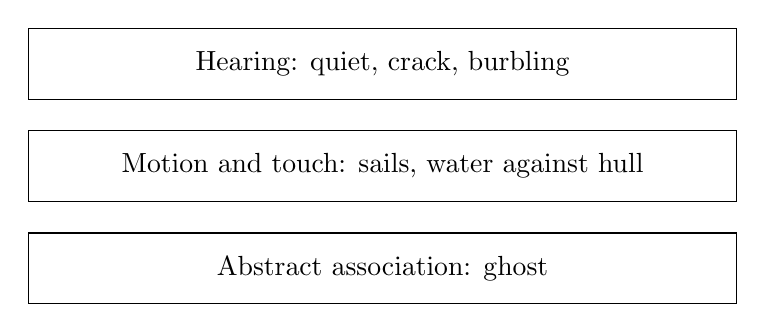
\begin{tikzpicture}
\node[draw, rectangle, minimum width=9cm, minimum height=0.9cm] (A) at (0,1.8) {Hearing: quiet, crack, burbling};
\node[draw, rectangle, minimum width=9cm, minimum height=0.9cm] (B) at (0,0.5) {Motion and touch: sails, water against hull};
\node[draw, rectangle, minimum width=9cm, minimum height=0.9cm] (C) at (0,-0.8) {Abstract association: ghost};
\end{tikzpicture}
\end{figure}

This transcript-based schematic is simple on purpose. It records the order in which the lecture itself unfolds the sentence: first sound, then movement and contact, then the abstract modifier that changes the atmosphere of the whole line.

\paragraph{Worked example.} The analytic order matters:
\begin{enumerate}
\item We isolate the sound-words: ``quiet,'' ``crack,'' ``burbling.''
\item We observe that these are specific acoustic qualities, not a generic class.
\item We then register motion and touch through sails and water against hull.
\item Only after that do we take in the abstract link between quiet and ghost.
\item The sentence works because these layers accumulate rather than substitute for one another.
\end{enumerate}

\subsection{Question \& Answer}

\paragraph{Question.} How does one sentence accumulate multiple sensory and conceptual layers?

\paragraph{Answer.} Because the words are not all serving the same function. Some sharpen sound, some imply movement or contact, and some create nonliteral association. A strong descriptive sentence distributes its labor across several registers and lets those registers reinforce one another.

\section{Metaphor, Simile, and Readerly Distance}

The next step is one of the lecture's most precise. The lecturer does not merely praise ``ghost quiet.'' She contrasts it with a nearby alternative: ``quiet as a ghost.'' The difference is not grammatical only. It changes the reader's relation to the scene:
\begin{align}
\text{quiet as a ghost} &\Rightarrow \text{greater distance},\\
\text{ghost quiet} &\Rightarrow \text{greater immediacy}.
\end{align}
The formal distinction may be written
\begin{align}
\text{simile} &\to \text{overt comparison},\\
\text{metaphor} &\to \text{implied comparison}.
\end{align}

We should keep the claim local. The lecture is not proving that metaphor always outranks simile. It is showing that in this instance the simile would insert an extra interpretive layer. We would be told more openly how to compare, and that explicitness would make us pause slightly outside the experience. ``Ghost quiet'' fuses the terms more tightly. The comparison happens within the phrase instead of being announced from above.

This is what the lecturer means by distance. One formulation lets us inspect the relation. The other lets us inhabit it more quickly.

\subsection{Question \& Answer}

\paragraph{Question.} What does simile add, and what distance does it impose?

\paragraph{Answer.} Simile adds explicitness. It makes the comparison unmistakable. That can be useful, but here it weakens immediacy by placing the reader one step farther from the sensation. The metaphor leaves the comparison implied and the scene more immediate.

\section{Against Clich\'e: Fresh Connotation and Reader Participation}

The lecture now turns from the local distinction between metaphor and simile to a broader problem: clich\'e. Writers are told to avoid overused images, and the lecture gives that advice real content:
\begin{equation}
\text{overused image} \Rightarrow \text{low reader engagement}.
\end{equation}
A phrase such as ``red as a rose'' demands very little. The comparison arrives already processed. The reader is not asked to do enough imaginative work.

The counterexample is equally exact. We are given the phrase ``stewed cherry dress.'' That phrase does not arrive complete. It makes the reader infer color, texture, density, even atmosphere. The image is not obscure; it is active. Hence the lecture's final relation:
\begin{equation}
\text{unexpected connotation} \to \text{reader participation} \to \text{immersion}.
\end{equation}
The reader is no longer just receiving description. The reader is helping to build the scene.

This is why the lecture closes with prescription rather than with theory. Use well-chosen words to engage sound, sight, taste, touch, smell, and movement. Then create unexpected connotations among the elements of the story. The final compression is
\begin{equation}
\text{sensory cue} + \text{fresh association} \Rightarrow \text{dynamic imaginative world}.
\end{equation}
The phrase about setting the reader's brushfire imagination alight is not an ornamental flourish. It is the endpoint of the argument. Description succeeds when it turns the reader from observer into participant.

\section{Summary}

The lecture moves in a strict sequence. We begin with why we read fiction and arrive at immersion as the governing standard. We then ask how prose can achieve that standard and test the answer against the Billy example, where vivid metaphor proves stronger than flat summary. From there we widen to a theory of prose as a medium of static symbols that must nevertheless produce sensory experience. The sentence about a world that was ``ghost quiet'' then becomes the lecture's worked example of layered description: hearing, motion, touch, and abstraction assembled in a single line. Finally, the lecture distinguishes metaphor from simile by the degree of distance each creates, warns against clich\'e, and shows why fresh connotation recruits the reader's imagination into the making of the scene. The result is a severe but practical lesson: description is one of the places where fiction converts language into lived experience.